\chapter{Connect Hydro Project}
\label{ChapterThree}



%As previously mentioned, the aim of the thesis is to propose a general offline synchronization framework for mobile devices. The current chapter presents the framework from the point of view of its architecture, characteristics and dependencies. An emphasis is put on the interaction between the components and their structure. 
%\section{Presentation of the Environment}
%\label{sec:EnvironmentPresentation}
%The problem addressed in this thesis concerns all applications running on different mobile operating systems. The common point of these applications is the dependency on a global database and their requirement of being able to be fully functional even in offline working mode.\\
%\indent Nowadays, most of the existing desktop applications have been extended with mobile ones that enable the user to interact with them from his gadget directly. Most of these mobile applications are tailored in such way that they are compliant with the characteristics of mobile devices. Design and development of mobile applications must be done accordingly to the infrastructure and technologies on top of which they are running. These aspects can concern either the information displayed in the GUI, either processing details that should take into consideration the limitations of the device.\\
%\indent Besides the restrictions imposed by the mobile technology there are some other aspects that enforce the applications. These new gadgets posses some abilities that cannot be retrieved on desktop computers. A very good example  is detecting the location of the user by using the GPS system. This functionality cannot be found on desktop applications yet. Nonetheless, the hardware structure facilitates functionality as the use of the camera, microphone, network connection that can allow applications to enrich the user experience with new interaction methods.\\
%\indent Using the camera to record and detect some information about physical objects or inputting the commands and data as voice instructions instead of normal text input make the human computer interaction more fluent and give these applications the ubiquitous character. The aim is to describe a general solution, therefore we will not make any assumptions on the possible extensions that can be added to the synchronization framework. In this way, a future developer can decide what extensions he would like to add to the system. The previous examples were given in order to emphasize the extensible character of mobile applications.\\
%\indent The framework proposed by this thesis is designed for such devices and must support besides its primary function of offline data synchronization some other mobile specific functionality as mentioned before. In the section dedicated to the architecture of the framework, other components that can be integrated in the case of specific solutions will be mentioned.
%\section{Detailed Design}
%\label{sec:Detailed Design}
%\indent The main area of focus is on the distributed applications on mobile devices. As mentioned in \cite{ModernOS2009}, the main architectural styles present in distributed system are the centralized and decentralized ones. The typical implementation for centralized model relies on a client - server architecture. In this model, the components of the system can fulfill one role: either they provide services and data being server components, either they request services or data being clients. The decentralized model relies on peer - to - peer implementations, be them structured on unstructured. Database replication and synchronization is more complex due to the decentralization \cite{Xhafa2012}. In the latter model, the architecture is decentralized and any component (peer) can either provide or request resources \cite{ModernOS2009}. From the two models, a third one, hybrid, has been developed. In the hybrid model, a central server permits the peers to find each other and afterwards exchange information between them.\\
%\indent As we are interested in Business to Business model (B2B), we have opted for developing a client - server solution. The choice is justified by the fact that the mobile application will mostly request data and services from the central server. Moreover, it runs on devices that can fulfill computational efforts for other parties. In client-server applications, the data is stored in central servers from which it can be accessed later on by the clients. Most of the information from the database is modified by the business supplier. However, some data is usually updated from the client side and sent further to the server. We will take a simple example for an application that stores information about clients and their orders. While the business supplier participant from the B2B model (server side) will handle all the information concerning the products and services they provide, the business consumer (client side) updates the data corresponding to it (client information, placed orders). All this information is centralized in a global database and periodic exchange of data is established between the client and the server side. A peer - to - peer model is undesirable in this case, as storing the data at different peers can endanger its safety and privacy. We will focus on the B2B model and therefore, on the client - server architecture.
%\subsection{System Architecture}
%\label{Architecture}
%\indent In order to understand how the components of the system must be connected and how the communication among them is established they must be first identified. The next step is to set the restrictions. The component diagram from figure 3.1 reveals the main parts of the system and how they are connected. 
%\subsubsection{Software Interfaces}
%\label{subsubsec:SoftwareInterfaces}
%\indent Software interfaces are shared boundaries between components of the system. By implementing them, the communication between the system components is performed through a layered architecture by using the paradigm of information hiding. In designing the software interface, we have to have in mind the fact that software changes and evolves frequently and the interfaces have to be built in such way that they can be easily customized in the future.\\
%\indent In order to identify the interface connectors, we have to define the components of the system. In the following part of the thesis, every component and connections between component will be taken individually and explained.
%\begin{figure}[ht]
%\centering
%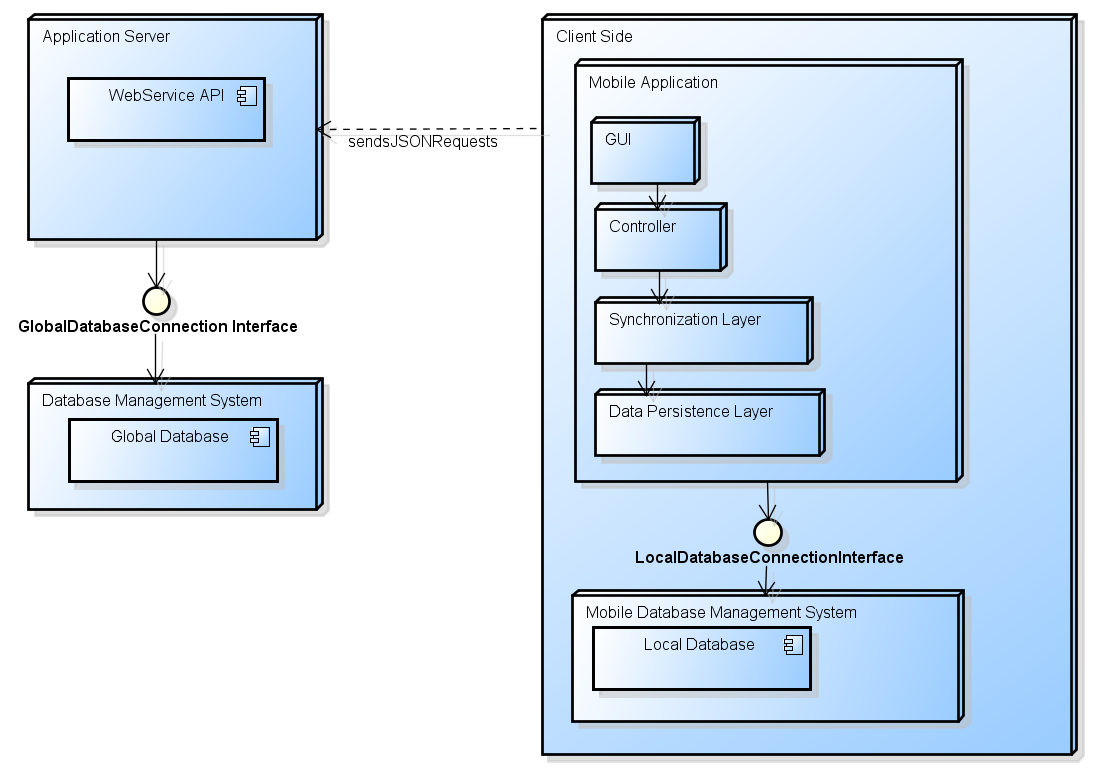
\includegraphics[scale=0.5]{Images/componentDiagram.png}
%\caption[System Component Diagram]{System Component Diagram}
%\end{figure}
%\begin{itemize}
%\item \textbf{Server component} - this component is responsible with storing the global database and handling the client requests. The underlying infrastructure is not limited to a certain technology. It can be a normal web application developed in different programming languages. The only restriction that is imposed on the server side is concerned with the database in which the information is stored. The databases that are considered viable for this framework are of relational type. As it can be seen further on, the interface between the server and the client component is more important as it has to deal with differences that can occur on both client and server side.
%\item \textbf{Client component} - this part of the system is the actual mobile application in which the synchronization mechanisms have to be deployed. It is independent of the running mobile operating system and has to contain certain components that are generalized so that they can be compliant with different mobile operating systems. The elements of this component and the way in which they are connected will be discussed in more details.
%\item \textbf{External components} - besides the client and server components, some external dependencies might be needed in order to ensure all the required functionality. For example, in the communication between the client and the server sides, a common protocol must be found. In case the data received at one side does not come in a standardized form, it must be parsed and transformed in specific data structures or objects that can be afterwards processed. Data parser is one example of external component that might be needed in order to ensure the complete and correct data flow inside the system. They were not presented in the diagram as they can vary from implementation to implementation.
%\end{itemize}
%\indent Knowing the main components of our system, the software interfaces that allow the communication among them can be defined.\\
%\indent Because the connection to the server side is in most of the cases Internet dependent the communication between the client and the server will occur with the aid of HTTP protocol. Now that the communication channel is established, a communication process description and language must be defined.\\
%\indent Dealing with distributed system, the most suitable architectural style for the communication between the client and the server components would be the Representational state transfer(REST) software architectural style. One of its main advantages rely in the fact that it is stateless, which means that the service calls can be load balanced and it enforces also the reliability non functional requirement. Other advantages are given by the capacity of being independent of the implementation and the protocol syntax and that it is focused mostly on the components' roles, interaction and processing of data elements\cite{Fielding2002principled}. REST technology was used among time for the implementation of web services. \\ 
%\indent The advantages brought by REST architectural style to our system are mostly based on its compatibility with the client - server architecture and the way in which it decouples both sides from the dependency on a certain implementation. Another important aspect facilitated by REST is the ability of the client to cache the responses obtained from the server on their requests. The caching process removes the permanent dependency on the server side and respectively on an Internet connection.
%\subsection{External Dependencies}
%\label{External Dependencies}
%The exchange of data between the client and the server component must be established. As seen previously, REST architecture does not constrain the development to a certain technology, but focuses on the role of the components. However, there are some dependencies on external libraries that must be mentioned. The aim is not to limit the dependencies to a certain technology so several possible options were considered, but only the one that seems more promising for our problem domain is described.
%\subsubsection{Communication Protocol}
%\label{CommunicationProtocol}
%The communication protocol between the client and the server side must allow both the components to exchange the data. As the server can be accessed from Internet, the rational choice for the communication protocol is HTTPS as it also supports security measures. HTTPS has eight methods each, but relies mostly on two main methods of requesting data: POST and GET\cite{Pautasso2008}. As the information sent from one side to the other can be private or public, the request method can be chosen accordingly: GET requests for public data and POST requests for private data.\\ Usually, the requests need some parameters that describe the information solicited. These parameters are sent together with the request and have to be expressed in a language that has to be understood from both sides. Therefore, the communication protocol relies on a common language of representing information. The aim of it is to create structured representations out of unstructured data. In this way the data from the source does not get changed on the target. Popular languages in this area are RDF, XML and JSON. As RDFs are limited to expressing the data in form of triples, we will mention some aspects only for the last two languages.\\
%\indent XML languages encodes the data in both human and machine - readable format in the form of embedded tags. It has been designed such that it can be used independently of the platform in a simple manner. Most of the programming languages have library that support parsing the data in XML format.\\
%\indent Another lightweight data exchange format is JSON. It supports the representation of data as collection of name value pairs that can store information for different object types and data structures and also can represent ordered list of values that are normally known in programming languages as arrays. By keeping the structure closed to the ones found in commonly used programming language the transition from such a format to data that can be integrated in a program is easy to do.\\
%\indent Opting for one despite of other is just a matter of preference and compatibility with the system in which the framework has to be deployed. Nonetheless, in order to extract the information from the raw data file and transform them into data structures, a parser library or a custom implementation of a parser is needed. Most of the existing programming languages were extended with parsing libraries for these data file types. 
%\subsection{Server Side Component}
%\label{ServerSide}
%The server side stores the global database and can be accessed from different client types: either normal web browsers or mobile devices running on various operating systems. REST architecture supports this assumption and imposes the server side only to provide an interface which will mediate the communication with the client. This interface must be responsible for receiving requests from the client side and passing further the requests to the responsible processing part.\\
%\indent The server side must be able to retrieve the data requested by the client (if it exists) and create a document for the communication language agreed with the client. It should be able to support different data exchange language types for different client types with which it works.\\
%\indent The most important action for the framework is the synchronization. In this step the communicating sides (the client and the server) try to resolve the existing conflicts occurring since the last synchronization time. As the pull requests are performed by the clients, the server must handle only the conflict resolution strategy. In the conflict resolution methods, the instances that are in inconsistent state are compared by fields. Those fields that are inconsistent are changed in the global database accordingly to the most recent version of the instance. The contents are replaced on the global database and the results of the conflict resolution strategy are sent back to the client so that it, in its turn, will be able to update the local database.\\
%\indent From the point of view of the client, the server side is like a black - box as no details on how the processing part is performed are known. The client is only aware of the interface as well as the communication protocol and the payload encryption format.
%\subsection{Client Side Component}
%\label{ClientSide}
%The client side component can vary from system to system as the requirements it has to fulfill are different. We will propose a layered structure of the application and describe the dependency between them and their role. The discussion will be supported by a component diagram.
%\begin{figure}[ht]
%\centering
%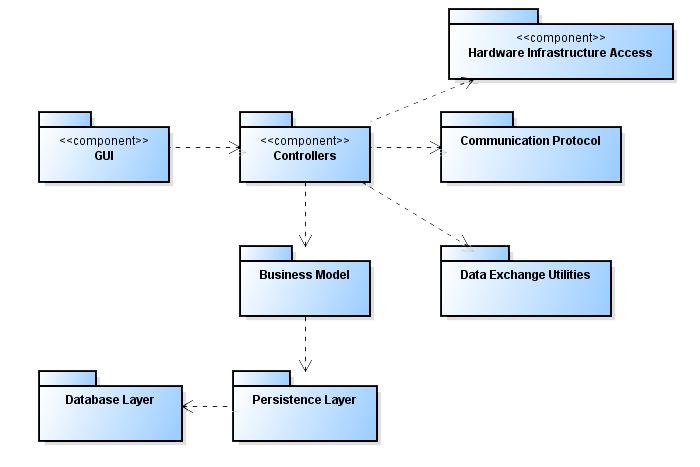
\includegraphics[scale=0.8]{Images/clientLayers.png}
%\caption[Client System Application Layers]{Client System Application Layers}
%\end{figure}
%\indent As we now have the schema of the main layers of the application, we will now analyze each of them, mentioning their role and constraints that have to be applied upon them. The dependencies among them can be depicted from the diagram 3.2, but we will mention their important aspects.\\
%\indent \textbf{GUI Component}. This part of the application contains the graphical interface with which the user interacts. It is not restricted to certain components and can vary from application to application. The aim is to design it by considering usability principles so it is straight - forward to use for both experienced and inexperienced users. As we are discussing the case of mobile applications, there are two main types of GUI solutions.\\
%\indent The first case is to build native applications by creating the GUI conform to the specifications of each type of programming language corresponding to the OS under which the device is running. The second option is to work with mobile frameworks that support the development of cross-platform applications. In the latter case, the performance is reduced than in the case of the native apps.\\
%\indent The GUI is responsible for displaying the information to the user and also capture his actions and send them to the controller. User's actions are monitored by registering listeners on the items with which he can interact. Whenever changes are performed in the database (e.g. after synchronization) the GUI has to be refreshed in order to display the latest version of the instances from the database. Refreshing the page is triggered from the controller whenever a process that can alter the database occurs.\\
%\indent This layer corresponds to the view component of the model - view - controller paradigm.\\
%\indent \textbf{Controllers}. As the name suggests, this layer corresponds to the controller layer from the model - view - controller paradigm. The application should rely on a main controller which in its turn manages other controllers responsible with a certain part of the system (e.g. synchronization, hardware controllers, data object processing). Being interested in having only one instance of them, the controllers are designed under the principles of singleton design pattern.\\
%\indent We will focus mainly on the controller responsible with the synchronization mechanism. On the first start of the application, the user has to authenticate himself in the system. After the authentication step, the controller will automatically request data synchronization. This synchronization is one of the most simple as it does not require any other computations. It just forwards the pull request of data to the server in order to obtain the data for the local database that corresponds to the logged in user. The parameter that allows this is the identifier of the user account that is logged in. This synchronization method relies on the same principles as the snapshot replication from SQL server databases.\\
%\indent The second type of synchronization aims to keep the information from the database in a consistent state and maintain it up-to-date. It relies on the assumption that information is found under the permanent process of change. As different systems have different velocities for changing the data they work it, it remains on the level of each implementation to decide what will be the frequency with which the synchronization process will be triggered. Of course, this process can be performed at different rates if the system is able to predict the number of changes in a certain interval and incrementally learn. As the database can contain a large number of instances it is undesirable to exchange it all. On the contrary, the aim is to update the information that might be out of date. As the client is responsible only for the pull requests, the server is responsible for detecting the data records that have been changed since the last synchronization. The records that are modified have a last update time stamp larger than the time stamp of the last synchronization. The controller from the client side sends the request to the server and the server replies with a document that contains the IDs of the data records that need to be synchronized. On the client side, the controller parses the list of records and requests them from the local database. A document with these records is sent to the server where the conflicts are solved. The result of the conflict resolution method is provided for both the client and server side, which update their database. Only the fields that were modified are updated. The time of this synchronization operation is recorded.\\
%\indent The last type of synchronization occurs is strongly dependent on the activity of the user on the mobile device. It is unrealistic to assume that the user has a permanent Internet connection. In case the mobile device stays offline for a certain period of time in which the user performs different operations that affect the database, it is necessary to send these changes to the server as soon as the device has an available Internet connection. Due to the fact that in most of the cases, only a part of the tables are affected by user's actions, the synchronization algorithm will handle those tables. In most of the cases, new records are inserted in the table (e.g. the user tries to store the products for an order in offline mode) and these records have to be sent to the server side. When the mobile device connects to Internet, a trigger for this type of synchronization is sent to the synchronization controller.\\
%\indent \textbf{Hardware Infrastructure Access}. In order to communicate to the hardware components and control them, an interface between the controllers and the hardware must be established. This layer is responsible with ensuring this communication. Depending on the components used, this layer requires different classes and communication protocols. The most frequent used hardware parts are the camera, the accelerometer and microphone but for example other sensors can bring important information depending on the system.\\
%\indent \textbf{Communication Protocol}. This part of the system is responsible with ensuring the communication of the client with the server. Inside this layer, a class that handles the network connection with the server is needed. Inside this class the communication protocol is initialized and all the authentication methods are defined. This class should contain also the methods responsible for creating the requests. The communication protocol is strongly correlated with the format of the data exchanged. Therefore, whenever a request has to be built in a certain format it calls the controller which in its turn calls the data exchange utilities methods. The connection to the server requests some security measures, reason for which it is important that on the client side authorization methods to be implemented.\\
%\indent \textbf{Data Exchange Utilities}. This layer strongly depends on the data exchange format chosen for the implementation. Knowing that and the data structure of the files that will be received, parsing methods have to be defined. The general parsing library is already constructed for different programming languages but it has to be used in various way according to the way in which the data schema has to be processed. This layer handles transformations of two types: either from object format to data exchange format, either the reverse. In the case the system receives data from the server and wants to store them in the database, this data has to be first transformed to an object and them persisted in the database. The conversion from the data format to the object format is handled by this layer. Reversely, if data has to be sent to the server, it is first retrieved from the database in the form of object instances. From these objects, a data exchange file has to be built. The classes that are part of this layer are responsible for handling the input/output flow and storing lightweight methods for converting information in different formats.\\
%\indent \textbf{Business Layer}. This layer contains the definition of the object classes involved in the application. The entities defined at this level are strongly correlated with the information stored in the database. This layer corresponds to the model from the model - view - controller paradigm. One class from this layer corresponds to one class in the database. Relationships from the database are defined as attributes of classes or different underlined with the aid of OOP concepts.\\
%\indent \textbf{Persistence Layer}. This layer handles all the methods needed to store the information in the database. It is responsible for creating all the queries needed to manipulate and extract the data from the database. This layer is used for extracting information from the database and creating object instances or persisting information from object instances to the database. It varies from system to system and from database schema to database schema.\\
%\indent \textbf{Database Layer}. This layer corresponds to the actual database component. In most of the cases, utility classes come already defined and they just need to be integrated in the system.
%\section{Performance Analysis}
%\label{sec:PerformanceAnalysis}
%The performance of this framework varies from system to system and it is strongly correlated with the implementation. However, having a general design proposed, the performances should be comparable. As there is not absolute measure for the general solution, we propose to test the results obtained by the particular implementation on an Android device presented in the fourth chapter. The analysis and the metrics used in interpreting the results are presented in fifth chapter.\\
%\indent Having the description of the general framework, we will move now further to presenting a version of its implementation on an Android application. More details will be given in the following chapter.